%% bm.pdf preamble - material merged from previous preamble and current pandoc preamable output
% NOTE: float placement required changes to the source files referenced by bm.tex
% May 28, 2020
%
% Use lualatex to compile - test with MiKTeX 2.9

% uncomment to list all files in log
%\listfiles

\documentclass[12pt]{report}


\usepackage{fontspec}

%\setmainfont[Scale=MatchLowercase]{Lucida Bright}
%\setmonofont{FreeMono}
%\setmonofont{Source Code Pro}
\setmonofont[Scale=MatchLowercase]{Ubuntu Mono}

% short snippets of asian languages
\newfontfamily\myAsian{Noto Serif TC Medium}

\usepackage[headings]{fullpage}

% national use characters 
%\usepackage{inputenc}

% ams mathematical symbols
\usepackage{amsmath,amssymb}

% added to support pandoc highlighting
\usepackage{microtype}

\usepackage{makeidx}

% add index and bibliographies to table of contents
\usepackage[nottoc]{tocbibind}

% postscript courier and times in place of cm fonts
%\usepackage{courier}
%\usepackage{times}

% extended coloring
\usepackage{color}
\usepackage[table,dvipsnames]{xcolor}
\usepackage{colortbl}

% advanced date formating
\usepackage{datetime}

%support pandoc code highlighting
\usepackage{fancyvrb}

% \DefineShortVerb[commandchars=\\\{\}]{\|}
% \DefineVerbatimEnvironment{Highlighting}{Verbatim}{commandchars=\\\{\}}
% % Add ',fontsize=\small' for more characters per line

% tango style colors
% \usepackage{framed}
% \definecolor{shadecolor}{RGB}{255,255,255}
% \newenvironment{Shaded}{\begin{snugshade}}{\end{snugshade}}
% \newcommand{\KeywordTok}[1]{\textcolor[rgb]{0.13,0.29,0.53}{\textbf{{#1}}}}
% \newcommand{\DataTypeTok}[1]{\textcolor[rgb]{0.13,0.29,0.53}{{#1}}}
% \newcommand{\DecValTok}[1]{\textcolor[rgb]{0.00,0.00,0.81}{{#1}}}
% \newcommand{\BaseNTok}[1]{\textcolor[rgb]{0.00,0.00,0.81}{{#1}}}
% \newcommand{\FloatTok}[1]{\textcolor[rgb]{0.00,0.00,0.81}{{#1}}}
% \newcommand{\CharTok}[1]{\textcolor[rgb]{0.31,0.60,0.02}{{#1}}}
% \newcommand{\StringTok}[1]{\textcolor[rgb]{0.31,0.60,0.02}{{#1}}}
% \newcommand{\CommentTok}[1]{\textcolor[rgb]{0.56,0.35,0.01}{\textit{{#1}}}}
% \newcommand{\OtherTok}[1]{\textcolor[rgb]{0.56,0.35,0.01}{{#1}}}
% \newcommand{\AlertTok}[1]{\textcolor[rgb]{0.94,0.16,0.16}{{#1}}}
% \newcommand{\FunctionTok}[1]{\textcolor[rgb]{0.00,0.00,0.00}{{#1}}}
% \newcommand{\RegionMarkerTok}[1]{{#1}}
% \newcommand{\ErrorTok}[1]{\textbf{{#1}}}
% \newcommand{\NormalTok}[1]{{#1}}

% %espresso style colors
% \usepackage{framed}
% \definecolor{shadecolor}{RGB}{42,33,28}
% \newenvironment{Shaded}{\begin{snugshade}}{\end{snugshade}}
% \newcommand{\KeywordTok}[1]{\textcolor[rgb]{0.26,0.66,0.93}{\textbf{{#1}}}}
% \newcommand{\DataTypeTok}[1]{\textcolor[rgb]{0.74,0.68,0.62}{\underline{{#1}}}}
% \newcommand{\DecValTok}[1]{\textcolor[rgb]{0.27,0.67,0.26}{{#1}}}
% \newcommand{\BaseNTok}[1]{\textcolor[rgb]{0.27,0.67,0.26}{{#1}}}
% \newcommand{\FloatTok}[1]{\textcolor[rgb]{0.27,0.67,0.26}{{#1}}}
% \newcommand{\CharTok}[1]{\textcolor[rgb]{0.02,0.61,0.04}{{#1}}}
% \newcommand{\StringTok}[1]{\textcolor[rgb]{0.02,0.61,0.04}{{#1}}}
% \newcommand{\CommentTok}[1]{\textcolor[rgb]{0.00,0.40,1.00}{\textit{{#1}}}}
% \newcommand{\OtherTok}[1]{\textcolor[rgb]{0.74,0.68,0.62}{{#1}}}
% \newcommand{\AlertTok}[1]{\textcolor[rgb]{1.00,1.00,0.00}{{#1}}}
% \newcommand{\FunctionTok}[1]{\textcolor[rgb]{1.00,0.58,0.35}{\textbf{{#1}}}}
% \newcommand{\RegionMarkerTok}[1]{\textcolor[rgb]{0.74,0.68,0.62}{{#1}}}
% \newcommand{\ErrorTok}[1]{\textcolor[rgb]{0.74,0.68,0.62}{\textbf{{#1}}}}
% \newcommand{\NormalTok}[1]{\textcolor[rgb]{0.74,0.68,0.62}{{#1}}}

% %kete style colors
% \newenvironment{Shaded}{}{}
% \newcommand{\KeywordTok}[1]{\textbf{{#1}}}
% \newcommand{\DataTypeTok}[1]{\textcolor[rgb]{0.50,0.00,0.00}{{#1}}}
% \newcommand{\DecValTok}[1]{\textcolor[rgb]{0.00,0.00,1.00}{{#1}}}
% \newcommand{\BaseNTok}[1]{\textcolor[rgb]{0.00,0.00,1.00}{{#1}}}
% \newcommand{\FloatTok}[1]{\textcolor[rgb]{0.50,0.00,0.50}{{#1}}}
% \newcommand{\CharTok}[1]{\textcolor[rgb]{1.00,0.00,1.00}{{#1}}}
% \newcommand{\StringTok}[1]{\textcolor[rgb]{0.87,0.00,0.00}{{#1}}}
% \newcommand{\CommentTok}[1]{\textcolor[rgb]{0.50,0.50,0.50}{\textit{{#1}}}}
% \newcommand{\OtherTok}[1]{{#1}}
% \newcommand{\AlertTok}[1]{\textcolor[rgb]{0.00,1.00,0.00}{\textbf{{#1}}}}
% \newcommand{\FunctionTok}[1]{\textcolor[rgb]{0.00,0.00,0.50}{{#1}}}
% \newcommand{\RegionMarkerTok}[1]{{#1}}
% \newcommand{\ErrorTok}[1]{\textcolor[rgb]{1.00,0.00,0.00}{\textbf{{#1}}}}
% \newcommand{\NormalTok}[1]{{#1}}
% %end pandoc code hacks

% jodliterate colors
\usepackage{color}
\definecolor{shadecolor}{RGB}{248,248,248}
% j control structures 
\definecolor{keywcolor}{rgb}{0.13,0.29,0.53}
% j explicit arguments x y m n u v
\definecolor{datacolor}{rgb}{0.13,0.29,0.53}
% j numbers - all types see j.xml
\definecolor{decvcolor}{rgb}{0.00,0.00,0.81}
\definecolor{basencolor}{rgb}{0.00,0.00,0.81}
\definecolor{floatcolor}{rgb}{0.00,0.00,0.81}
% j local assignments
\definecolor{charcolor}{rgb}{0.31,0.60,0.02}
\definecolor{stringcolor}{rgb}{0.31,0.60,0.02}
\definecolor{commentcolor}{rgb}{0.56,0.35,0.01}
% primitive adverbs and conjunctions
%\definecolor{othercolor}{rgb}{0.56,0.35,0.01}   
\definecolor{othercolor}{RGB}{0,0,255}
% global assignments
\definecolor{alertcolor}{rgb}{0.94,0.16,0.16}
% primitive J verbs and noun names
\definecolor{funccolor}{rgb}{0.00,0.00,0.00}

% custom colors
\definecolor{CodeBackGround}{cmyk}{0.0,0.0,0,0.05}    % light gray
\definecolor{CodeComment}{rgb}{0,0.50,0.00}           % dark green {0,0.45,0.08}
\definecolor{TableStripes}{gray}{0.9}                 % odd/even background in tables

% Colors for the hyperref package
\definecolor{urlcolor}{rgb}{0,.145,.698}
\definecolor{linkcolor}{rgb}{.71,0.21,0.01}
\definecolor{citecolor}{rgb}{.12,.54,.11}

% % Exact colors from NB
\definecolor{incolor}{HTML}{303F9F}
\definecolor{outcolor}{HTML}{D84315}
\definecolor{cellborder}{HTML}{CFCFCF}
\definecolor{cellbackground}{HTML}{F7F7F7}

% % ANSI colors
\definecolor{ansi-black}{HTML}{3E424D}
\definecolor{ansi-black-intense}{HTML}{282C36}
\definecolor{ansi-red}{HTML}{E75C58}
\definecolor{ansi-red-intense}{HTML}{B22B31}
\definecolor{ansi-green}{HTML}{00A250}
\definecolor{ansi-green-intense}{HTML}{007427}
\definecolor{ansi-yellow}{HTML}{DDB62B}
\definecolor{ansi-yellow-intense}{HTML}{B27D12}
\definecolor{ansi-blue}{HTML}{208FFB}
\definecolor{ansi-blue-intense}{HTML}{0065CA}
\definecolor{ansi-magenta}{HTML}{D160C4}
\definecolor{ansi-magenta-intense}{HTML}{A03196}
\definecolor{ansi-cyan}{HTML}{60C6C8}
\definecolor{ansi-cyan-intense}{HTML}{258F8F}
\definecolor{ansi-white}{HTML}{C5C1B4}
\definecolor{ansi-white-intense}{HTML}{A1A6B2}
\definecolor{ansi-default-inverse-fg}{HTML}{FFFFFF}
\definecolor{ansi-default-inverse-bg}{HTML}{000000}
    

% \usepackage{framed}
% \newenvironment{Shaded}{}{}
% \newcommand{\KeywordTok}[1]{\textcolor{keywcolor}{\textbf{{#1}}}}
% \newcommand{\DataTypeTok}[1]{\textcolor{datacolor}{{#1}}}
% %\newcommand{\DecValTok}[1]{\textcolor{decvcolor}{{#1}}}
% \newcommand{\DecValTok}[1]{{#1}} 
% \newcommand{\BaseNTok}[1]{\textcolor{basencolor}{{#1}}}
% \newcommand{\FloatTok}[1]{\textcolor{floatcolor}{{#1}}}
% \newcommand{\CharTok}[1]{\textcolor{charcolor}{\textbf{{#1}}}}
% \newcommand{\StringTok}[1]{\textcolor{stringcolor}{{#1}}}
% \newcommand{\CommentTok}[1]{\textcolor{commentcolor}{\textit{{#1}}}}
% \newcommand{\OtherTok}[1]{\textcolor{othercolor}{{#1}}} 
% \newcommand{\AlertTok}[1]{\textcolor{alertcolor}{\textbf{{#1}}}}
% %\newcommand{\FunctionTok}[1]{\textcolor{funccolor}{{#1}}}
% \newcommand{\FunctionTok}[1]{{#1}}
% \newcommand{\RegionMarkerTok}[1]{{#1}}
% \newcommand{\ErrorTok}[1]{\textbf{{#1}}}
% \newcommand{\NormalTok}[1]{{#1}}

% The default LaTeX title has an obnoxious amount of whitespace. By default,
% titling removes some of it. It also provides customization options.
\usepackage{titling}

% headers and footers
\usepackage{fancyhdr}
%\pagestyle{fancy}
\pagestyle{plain}

\fancyhead{}
\fancyfoot{}

%\fancyhead[LE,RO]{\slshape \rightmark}
%\fancyhead[LO,RE]{\slshape \leftmark}
\fancyfoot[C]{\thepage}
%\headrulewidth 0.4pt
%\footrulewidth 0 pt

%\addtolength{\headheight}{\baselineskip}

%\lfoot{\emph{Analyze the Data not the Drivel}}
%\rfoot{\emph{\today}}

% subfigure handles figures that contain subfigures
%\usepackage{color,graphicx,subfigure,sidecap}
\usepackage{graphicx,sidecap}
\usepackage{subfigure}
\graphicspath{{./inclusions/}}

% floatflt provides for text wrapping around small figures and tables
\usepackage{floatflt}

% tweak caption formats 
\usepackage{caption} 
\usepackage{sidecap}
%\usepackage{subcaption} % not compatible with subfigure

\usepackage{rotating} % flip tables sideways

% complex footnotes
%\usepackage{bigfoot}

% weird logos \XeLaTeX
\usepackage{metalogo}

\newcommand{\HRule}{\rule{\linewidth}{0.5mm}}

\usepackage[breakable]{tcolorbox}

\usepackage{parskip} % Stop auto-indenting (to mimic markdown behaviour)
    
% Basic figure setup, for now with no caption control since it's done
% automatically by Pandoc (which extracts ![](path) syntax from Markdown).
\usepackage{graphicx}

%\DeclareCaptionFormat{nocaption}{}
%\captionsetup{format=nocaption,aboveskip=0pt,belowskip=0pt}

\usepackage[Export]{adjustbox} % Used to constrain images to a maximum size
\adjustboxset{max size={0.9\linewidth}{0.9\paperheight}}
\usepackage{float}

%\floatplacement{figure}{H} % forces figures to be placed at the correct location

\usepackage{xcolor} % Allow colors to be defined
\usepackage{enumerate} % Needed for markdown enumerations to work
\usepackage{geometry} % Used to adjust the document margins

%\usepackage{amsmath} % Equations
%\usepackage{amssymb} % Equations

\usepackage{textcomp} % defines textquotesingle

% Hack from http://tex.stackexchange.com/a/47451/13684:
\AtBeginDocument{%
	\def\PYZsq{\textquotesingle}% Upright quotes in Pygmentized code
}

\usepackage{upquote} % Upright quotes for verbatim code
\usepackage{eurosym} % defines \euro
\usepackage[mathletters]{ucs} % Extended unicode (utf-8) support

%\usepackage{fancyvrb} % verbatim replacement that allows latex

\usepackage{grffile} % extends the file name processing of package graphics 
					 % to support a larger range
					 
\makeatletter % fix for grffile with XeLaTeX
\def\Gread@@xetex#1{%
  \IfFileExists{"\Gin@base".bb}%
  {\Gread@eps{\Gin@base.bb}}%
  {\Gread@@xetex@aux#1}%
}
\makeatother

% The hyperref package gives us a pdf with properly built
% internal navigation ('pdf bookmarks' for the table of contents,
% internal cross-reference links, web links for URLs, etc.)
\usepackage{hyperref}
% The default LaTeX title has an obnoxious amount of whitespace. By default,
% titling removes some of it. It also provides customization options.
\usepackage{titling}
\usepackage{longtable} % longtable support required by pandoc >1.10
\usepackage{booktabs}  % table support for pandoc > 1.12.2
\usepackage[inline]{enumitem} % IRkernel/repr support (it uses the enumerate* environment)
\usepackage[normalem]{ulem} % ulem is needed to support strikethroughs (\sout)
							% normalem makes italics be italics, not underlines
\usepackage{mathrsfs}

% commands and environments needed by pandoc snippets
% extracted from the output of `pandoc -s`
\providecommand{\tightlist}{%
  \setlength{\itemsep}{0pt}\setlength{\parskip}{0pt}}
  
\DefineVerbatimEnvironment{Highlighting}{Verbatim}{commandchars=\\\{\}}
% Add ',fontsize=\small' for more characters per line
\newenvironment{Shaded}{}{}
\newcommand{\KeywordTok}[1]{\textcolor[rgb]{0.00,0.44,0.13}{\textbf{{#1}}}}
\newcommand{\DataTypeTok}[1]{\textcolor[rgb]{0.56,0.13,0.00}{{#1}}}
\newcommand{\DecValTok}[1]{\textcolor[rgb]{0.25,0.63,0.44}{{#1}}}
\newcommand{\BaseNTok}[1]{\textcolor[rgb]{0.25,0.63,0.44}{{#1}}}
\newcommand{\FloatTok}[1]{\textcolor[rgb]{0.25,0.63,0.44}{{#1}}}
\newcommand{\CharTok}[1]{\textcolor[rgb]{0.25,0.44,0.63}{{#1}}}
\newcommand{\StringTok}[1]{\textcolor[rgb]{0.25,0.44,0.63}{{#1}}}
\newcommand{\CommentTok}[1]{\textcolor[rgb]{0.38,0.63,0.69}{\textit{{#1}}}}
\newcommand{\OtherTok}[1]{\textcolor[rgb]{0.00,0.44,0.13}{{#1}}}
\newcommand{\AlertTok}[1]{\textcolor[rgb]{1.00,0.00,0.00}{\textbf{{#1}}}}
\newcommand{\FunctionTok}[1]{\textcolor[rgb]{0.02,0.16,0.49}{{#1}}}
\newcommand{\RegionMarkerTok}[1]{{#1}}
\newcommand{\ErrorTok}[1]{\textcolor[rgb]{1.00,0.00,0.00}{\textbf{{#1}}}}
\newcommand{\NormalTok}[1]{{#1}}

% Additional commands for more recent versions of Pandoc
\newcommand{\ConstantTok}[1]{\textcolor[rgb]{0.53,0.00,0.00}{{#1}}}
\newcommand{\SpecialCharTok}[1]{\textcolor[rgb]{0.25,0.44,0.63}{{#1}}}
\newcommand{\VerbatimStringTok}[1]{\textcolor[rgb]{0.25,0.44,0.63}{{#1}}}
\newcommand{\SpecialStringTok}[1]{\textcolor[rgb]{0.73,0.40,0.53}{{#1}}}
\newcommand{\ImportTok}[1]{{#1}}
\newcommand{\DocumentationTok}[1]{\textcolor[rgb]{0.73,0.13,0.13}{\textit{{#1}}}}
\newcommand{\AnnotationTok}[1]{\textcolor[rgb]{0.38,0.63,0.69}{\textbf{\textit{{#1}}}}}
\newcommand{\CommentVarTok}[1]{\textcolor[rgb]{0.38,0.63,0.69}{\textbf{\textit{{#1}}}}}
\newcommand{\VariableTok}[1]{\textcolor[rgb]{0.10,0.09,0.49}{{#1}}}
\newcommand{\ControlFlowTok}[1]{\textcolor[rgb]{0.00,0.44,0.13}{\textbf{{#1}}}}
\newcommand{\OperatorTok}[1]{\textcolor[rgb]{0.40,0.40,0.40}{{#1}}}
\newcommand{\BuiltInTok}[1]{{#1}}
\newcommand{\ExtensionTok}[1]{{#1}}
\newcommand{\PreprocessorTok}[1]{\textcolor[rgb]{0.74,0.48,0.00}{{#1}}}
\newcommand{\AttributeTok}[1]{\textcolor[rgb]{0.49,0.56,0.16}{{#1}}}
\newcommand{\InformationTok}[1]{\textcolor[rgb]{0.38,0.63,0.69}{\textbf{\textit{{#1}}}}}
\newcommand{\WarningTok}[1]{\textcolor[rgb]{0.38,0.63,0.69}{\textbf{\textit{{#1}}}}}

% Define a nice break command that doesn't care if a line doesn't already exist.
\def\br{\hspace*{\fill} \\* }
% Math Jax compatibility definitions
\def\gt{>}
\def\lt{<}
\let\Oldtex\TeX
\let\Oldlatex\LaTeX
\renewcommand{\TeX}{\textrm{\Oldtex}}
\renewcommand{\LaTeX}{\textrm{\Oldlatex}}
 
% Pygments definitions
\makeatletter
\def\PY@reset{\let\PY@it=\relax \let\PY@bf=\relax%
    \let\PY@ul=\relax \let\PY@tc=\relax%
    \let\PY@bc=\relax \let\PY@ff=\relax}
\def\PY@tok#1{\csname PY@tok@#1\endcsname}
\def\PY@toks#1+{\ifx\relax#1\empty\else%
    \PY@tok{#1}\expandafter\PY@toks\fi}
\def\PY@do#1{\PY@bc{\PY@tc{\PY@ul{%
    \PY@it{\PY@bf{\PY@ff{#1}}}}}}}
\def\PY#1#2{\PY@reset\PY@toks#1+\relax+\PY@do{#2}}

\expandafter\def\csname PY@tok@w\endcsname{\def\PY@tc##1{\textcolor[rgb]{0.73,0.73,0.73}{##1}}}
\expandafter\def\csname PY@tok@c\endcsname{\let\PY@it=\textit\def\PY@tc##1{\textcolor[rgb]{0.25,0.50,0.50}{##1}}}
\expandafter\def\csname PY@tok@cp\endcsname{\def\PY@tc##1{\textcolor[rgb]{0.74,0.48,0.00}{##1}}}
\expandafter\def\csname PY@tok@k\endcsname{\let\PY@bf=\textbf\def\PY@tc##1{\textcolor[rgb]{0.00,0.50,0.00}{##1}}}
\expandafter\def\csname PY@tok@kp\endcsname{\def\PY@tc##1{\textcolor[rgb]{0.00,0.50,0.00}{##1}}}
\expandafter\def\csname PY@tok@kt\endcsname{\def\PY@tc##1{\textcolor[rgb]{0.69,0.00,0.25}{##1}}}
\expandafter\def\csname PY@tok@o\endcsname{\def\PY@tc##1{\textcolor[rgb]{0.40,0.40,0.40}{##1}}}
\expandafter\def\csname PY@tok@ow\endcsname{\let\PY@bf=\textbf\def\PY@tc##1{\textcolor[rgb]{0.67,0.13,1.00}{##1}}}
\expandafter\def\csname PY@tok@nb\endcsname{\def\PY@tc##1{\textcolor[rgb]{0.00,0.50,0.00}{##1}}}
\expandafter\def\csname PY@tok@nf\endcsname{\def\PY@tc##1{\textcolor[rgb]{0.00,0.00,1.00}{##1}}}
\expandafter\def\csname PY@tok@nc\endcsname{\let\PY@bf=\textbf\def\PY@tc##1{\textcolor[rgb]{0.00,0.00,1.00}{##1}}}
\expandafter\def\csname PY@tok@nn\endcsname{\let\PY@bf=\textbf\def\PY@tc##1{\textcolor[rgb]{0.00,0.00,1.00}{##1}}}
\expandafter\def\csname PY@tok@ne\endcsname{\let\PY@bf=\textbf\def\PY@tc##1{\textcolor[rgb]{0.82,0.25,0.23}{##1}}}
\expandafter\def\csname PY@tok@nv\endcsname{\def\PY@tc##1{\textcolor[rgb]{0.10,0.09,0.49}{##1}}}
\expandafter\def\csname PY@tok@no\endcsname{\def\PY@tc##1{\textcolor[rgb]{0.53,0.00,0.00}{##1}}}
\expandafter\def\csname PY@tok@nl\endcsname{\def\PY@tc##1{\textcolor[rgb]{0.63,0.63,0.00}{##1}}}
\expandafter\def\csname PY@tok@ni\endcsname{\let\PY@bf=\textbf\def\PY@tc##1{\textcolor[rgb]{0.60,0.60,0.60}{##1}}}
\expandafter\def\csname PY@tok@na\endcsname{\def\PY@tc##1{\textcolor[rgb]{0.49,0.56,0.16}{##1}}}
\expandafter\def\csname PY@tok@nt\endcsname{\let\PY@bf=\textbf\def\PY@tc##1{\textcolor[rgb]{0.00,0.50,0.00}{##1}}}
\expandafter\def\csname PY@tok@nd\endcsname{\def\PY@tc##1{\textcolor[rgb]{0.67,0.13,1.00}{##1}}}
\expandafter\def\csname PY@tok@s\endcsname{\def\PY@tc##1{\textcolor[rgb]{0.73,0.13,0.13}{##1}}}
\expandafter\def\csname PY@tok@sd\endcsname{\let\PY@it=\textit\def\PY@tc##1{\textcolor[rgb]{0.73,0.13,0.13}{##1}}}
\expandafter\def\csname PY@tok@si\endcsname{\let\PY@bf=\textbf\def\PY@tc##1{\textcolor[rgb]{0.73,0.40,0.53}{##1}}}
\expandafter\def\csname PY@tok@se\endcsname{\let\PY@bf=\textbf\def\PY@tc##1{\textcolor[rgb]{0.73,0.40,0.13}{##1}}}
\expandafter\def\csname PY@tok@sr\endcsname{\def\PY@tc##1{\textcolor[rgb]{0.73,0.40,0.53}{##1}}}
\expandafter\def\csname PY@tok@ss\endcsname{\def\PY@tc##1{\textcolor[rgb]{0.10,0.09,0.49}{##1}}}
\expandafter\def\csname PY@tok@sx\endcsname{\def\PY@tc##1{\textcolor[rgb]{0.00,0.50,0.00}{##1}}}
\expandafter\def\csname PY@tok@m\endcsname{\def\PY@tc##1{\textcolor[rgb]{0.40,0.40,0.40}{##1}}}
\expandafter\def\csname PY@tok@gh\endcsname{\let\PY@bf=\textbf\def\PY@tc##1{\textcolor[rgb]{0.00,0.00,0.50}{##1}}}
\expandafter\def\csname PY@tok@gu\endcsname{\let\PY@bf=\textbf\def\PY@tc##1{\textcolor[rgb]{0.50,0.00,0.50}{##1}}}
\expandafter\def\csname PY@tok@gd\endcsname{\def\PY@tc##1{\textcolor[rgb]{0.63,0.00,0.00}{##1}}}
\expandafter\def\csname PY@tok@gi\endcsname{\def\PY@tc##1{\textcolor[rgb]{0.00,0.63,0.00}{##1}}}
\expandafter\def\csname PY@tok@gr\endcsname{\def\PY@tc##1{\textcolor[rgb]{1.00,0.00,0.00}{##1}}}
\expandafter\def\csname PY@tok@ge\endcsname{\let\PY@it=\textit}
\expandafter\def\csname PY@tok@gs\endcsname{\let\PY@bf=\textbf}
\expandafter\def\csname PY@tok@gp\endcsname{\let\PY@bf=\textbf\def\PY@tc##1{\textcolor[rgb]{0.00,0.00,0.50}{##1}}}
\expandafter\def\csname PY@tok@go\endcsname{\def\PY@tc##1{\textcolor[rgb]{0.53,0.53,0.53}{##1}}}
\expandafter\def\csname PY@tok@gt\endcsname{\def\PY@tc##1{\textcolor[rgb]{0.00,0.27,0.87}{##1}}}
\expandafter\def\csname PY@tok@err\endcsname{\def\PY@bc##1{\setlength{\fboxsep}{0pt}\fcolorbox[rgb]{1.00,0.00,0.00}{1,1,1}{\strut ##1}}}
\expandafter\def\csname PY@tok@kc\endcsname{\let\PY@bf=\textbf\def\PY@tc##1{\textcolor[rgb]{0.00,0.50,0.00}{##1}}}
\expandafter\def\csname PY@tok@kd\endcsname{\let\PY@bf=\textbf\def\PY@tc##1{\textcolor[rgb]{0.00,0.50,0.00}{##1}}}
\expandafter\def\csname PY@tok@kn\endcsname{\let\PY@bf=\textbf\def\PY@tc##1{\textcolor[rgb]{0.00,0.50,0.00}{##1}}}
\expandafter\def\csname PY@tok@kr\endcsname{\let\PY@bf=\textbf\def\PY@tc##1{\textcolor[rgb]{0.00,0.50,0.00}{##1}}}
\expandafter\def\csname PY@tok@bp\endcsname{\def\PY@tc##1{\textcolor[rgb]{0.00,0.50,0.00}{##1}}}
\expandafter\def\csname PY@tok@fm\endcsname{\def\PY@tc##1{\textcolor[rgb]{0.00,0.00,1.00}{##1}}}
\expandafter\def\csname PY@tok@vc\endcsname{\def\PY@tc##1{\textcolor[rgb]{0.10,0.09,0.49}{##1}}}
\expandafter\def\csname PY@tok@vg\endcsname{\def\PY@tc##1{\textcolor[rgb]{0.10,0.09,0.49}{##1}}}
\expandafter\def\csname PY@tok@vi\endcsname{\def\PY@tc##1{\textcolor[rgb]{0.10,0.09,0.49}{##1}}}
\expandafter\def\csname PY@tok@vm\endcsname{\def\PY@tc##1{\textcolor[rgb]{0.10,0.09,0.49}{##1}}}
\expandafter\def\csname PY@tok@sa\endcsname{\def\PY@tc##1{\textcolor[rgb]{0.73,0.13,0.13}{##1}}}
\expandafter\def\csname PY@tok@sb\endcsname{\def\PY@tc##1{\textcolor[rgb]{0.73,0.13,0.13}{##1}}}
\expandafter\def\csname PY@tok@sc\endcsname{\def\PY@tc##1{\textcolor[rgb]{0.73,0.13,0.13}{##1}}}
\expandafter\def\csname PY@tok@dl\endcsname{\def\PY@tc##1{\textcolor[rgb]{0.73,0.13,0.13}{##1}}}
\expandafter\def\csname PY@tok@s2\endcsname{\def\PY@tc##1{\textcolor[rgb]{0.73,0.13,0.13}{##1}}}
\expandafter\def\csname PY@tok@sh\endcsname{\def\PY@tc##1{\textcolor[rgb]{0.73,0.13,0.13}{##1}}}
\expandafter\def\csname PY@tok@s1\endcsname{\def\PY@tc##1{\textcolor[rgb]{0.73,0.13,0.13}{##1}}}
\expandafter\def\csname PY@tok@mb\endcsname{\def\PY@tc##1{\textcolor[rgb]{0.40,0.40,0.40}{##1}}}
\expandafter\def\csname PY@tok@mf\endcsname{\def\PY@tc##1{\textcolor[rgb]{0.40,0.40,0.40}{##1}}}
\expandafter\def\csname PY@tok@mh\endcsname{\def\PY@tc##1{\textcolor[rgb]{0.40,0.40,0.40}{##1}}}
\expandafter\def\csname PY@tok@mi\endcsname{\def\PY@tc##1{\textcolor[rgb]{0.40,0.40,0.40}{##1}}}
\expandafter\def\csname PY@tok@il\endcsname{\def\PY@tc##1{\textcolor[rgb]{0.40,0.40,0.40}{##1}}}
\expandafter\def\csname PY@tok@mo\endcsname{\def\PY@tc##1{\textcolor[rgb]{0.40,0.40,0.40}{##1}}}
\expandafter\def\csname PY@tok@ch\endcsname{\let\PY@it=\textit\def\PY@tc##1{\textcolor[rgb]{0.25,0.50,0.50}{##1}}}
\expandafter\def\csname PY@tok@cm\endcsname{\let\PY@it=\textit\def\PY@tc##1{\textcolor[rgb]{0.25,0.50,0.50}{##1}}}
\expandafter\def\csname PY@tok@cpf\endcsname{\let\PY@it=\textit\def\PY@tc##1{\textcolor[rgb]{0.25,0.50,0.50}{##1}}}
\expandafter\def\csname PY@tok@c1\endcsname{\let\PY@it=\textit\def\PY@tc##1{\textcolor[rgb]{0.25,0.50,0.50}{##1}}}
\expandafter\def\csname PY@tok@cs\endcsname{\let\PY@it=\textit\def\PY@tc##1{\textcolor[rgb]{0.25,0.50,0.50}{##1}}}

\def\PYZbs{\char`\\}
\def\PYZus{\char`\_}
\def\PYZob{\char`\{}
\def\PYZcb{\char`\}}
\def\PYZca{\char`\^}
\def\PYZam{\char`\&}
\def\PYZlt{\char`\<}
\def\PYZgt{\char`\>}
\def\PYZsh{\char`\#}
\def\PYZpc{\char`\%}
\def\PYZdl{\char`\$}
\def\PYZhy{\char`\-}
\def\PYZsq{\char`\'}
\def\PYZdq{\char`\"}
\def\PYZti{\char`\~}
% for compatibility with earlier versions
\def\PYZat{@}
\def\PYZlb{[}
\def\PYZrb{]}
\makeatother

% For linebreaks inside Verbatim environment from package fancyvrb. 
\makeatletter
	\newbox\Wrappedcontinuationbox 
	\newbox\Wrappedvisiblespacebox 
	\newcommand*\Wrappedvisiblespace {\textcolor{red}{\textvisiblespace}} 
	\newcommand*\Wrappedcontinuationsymbol {\textcolor{red}{\llap{\tiny$\m@th\hookrightarrow$}}} 
	\newcommand*\Wrappedcontinuationindent {3ex } 
	\newcommand*\Wrappedafterbreak {\kern\Wrappedcontinuationindent\copy\Wrappedcontinuationbox} 
	% Take advantage of the already applied Pygments mark-up to insert 
	% potential linebreaks for TeX processing. 
	%        {, <, #, %, $, ' and ": go to next line. 
	%        _, }, ^, &, >, - and ~: stay at end of broken line. 
	% Use of \textquotesingle for straight quote. 
	\newcommand*\Wrappedbreaksatspecials {% 
		\def\PYGZus{\discretionary{\char`\_}{\Wrappedafterbreak}{\char`\_}}% 
		\def\PYGZob{\discretionary{}{\Wrappedafterbreak\char`\{}{\char`\{}}% 
		\def\PYGZcb{\discretionary{\char`\}}{\Wrappedafterbreak}{\char`\}}}% 
		\def\PYGZca{\discretionary{\char`\^}{\Wrappedafterbreak}{\char`\^}}% 
		\def\PYGZam{\discretionary{\char`\&}{\Wrappedafterbreak}{\char`\&}}% 
		\def\PYGZlt{\discretionary{}{\Wrappedafterbreak\char`\<}{\char`\<}}% 
		\def\PYGZgt{\discretionary{\char`\>}{\Wrappedafterbreak}{\char`\>}}% 
		\def\PYGZsh{\discretionary{}{\Wrappedafterbreak\char`\#}{\char`\#}}% 
		\def\PYGZpc{\discretionary{}{\Wrappedafterbreak\char`\%}{\char`\%}}% 
		\def\PYGZdl{\discretionary{}{\Wrappedafterbreak\char`\$}{\char`\$}}% 
		\def\PYGZhy{\discretionary{\char`\-}{\Wrappedafterbreak}{\char`\-}}% 
		\def\PYGZsq{\discretionary{}{\Wrappedafterbreak\textquotesingle}{\textquotesingle}}% 
		\def\PYGZdq{\discretionary{}{\Wrappedafterbreak\char`\"}{\char`\"}}% 
		\def\PYGZti{\discretionary{\char`\~}{\Wrappedafterbreak}{\char`\~}}% 
	} 
	% Some characters . , ; ? ! / are not pygmentized. 
	% This macro makes them "active" and they will insert potential linebreaks 
	\newcommand*\Wrappedbreaksatpunct {% 
		\lccode`\~`\.\lowercase{\def~}{\discretionary{\hbox{\char`\.}}{\Wrappedafterbreak}{\hbox{\char`\.}}}% 
		\lccode`\~`\,\lowercase{\def~}{\discretionary{\hbox{\char`\,}}{\Wrappedafterbreak}{\hbox{\char`\,}}}% 
		\lccode`\~`\;\lowercase{\def~}{\discretionary{\hbox{\char`\;}}{\Wrappedafterbreak}{\hbox{\char`\;}}}% 
		\lccode`\~`\:\lowercase{\def~}{\discretionary{\hbox{\char`\:}}{\Wrappedafterbreak}{\hbox{\char`\:}}}% 
		\lccode`\~`\?\lowercase{\def~}{\discretionary{\hbox{\char`\?}}{\Wrappedafterbreak}{\hbox{\char`\?}}}% 
		\lccode`\~`\!\lowercase{\def~}{\discretionary{\hbox{\char`\!}}{\Wrappedafterbreak}{\hbox{\char`\!}}}% 
		\lccode`\~`\/\lowercase{\def~}{\discretionary{\hbox{\char`\/}}{\Wrappedafterbreak}{\hbox{\char`\/}}}% 
		\catcode`\.\active
		\catcode`\,\active 
		\catcode`\;\active
		\catcode`\:\active
		\catcode`\?\active
		\catcode`\!\active
		\catcode`\/\active 
		\lccode`\~`\~ 	
	}
\makeatother

\let\OriginalVerbatim=\Verbatim
\makeatletter
\renewcommand{\Verbatim}[1][1]{%
	%\parskip\z@skip
	\sbox\Wrappedcontinuationbox {\Wrappedcontinuationsymbol}%
	\sbox\Wrappedvisiblespacebox {\FV@SetupFont\Wrappedvisiblespace}%
	\def\FancyVerbFormatLine ##1{\hsize\linewidth
		\vtop{\raggedright\hyphenpenalty\z@\exhyphenpenalty\z@
			\doublehyphendemerits\z@\finalhyphendemerits\z@
			\strut ##1\strut}%
	}%
	% If the linebreak is at a space, the latter will be displayed as visible
	% space at end of first line, and a continuation symbol starts next line.
	% Stretch/shrink are however usually zero for typewriter font.
	\def\FV@Space {%
		\nobreak\hskip\z@ plus\fontdimen3\font minus\fontdimen4\font
		\discretionary{\copy\Wrappedvisiblespacebox}{\Wrappedafterbreak}
		{\kern\fontdimen2\font}%
	}%
	
	% Allow breaks at special characters using \PYG... macros.
	\Wrappedbreaksatspecials
	% Breaks at punctuation characters . , ; ? ! and / need catcode=\active 	
	\OriginalVerbatim[#1,codes*=\Wrappedbreaksatpunct]%
}
\makeatother


% prompt
\makeatletter
\newcommand{\boxspacing}{\kern\kvtcb@left@rule\kern\kvtcb@boxsep}
\makeatother
\newcommand{\prompt}[4]{
	\ttfamily\llap{{\color{#2}[#3]:\hspace{3pt}#4}}\vspace{-\baselineskip}
}
    

% Prevent overflowing lines due to hard-to-break entities
\sloppy 

% Setup hyperref package
\hypersetup{
  breaklinks=true,  % so long urls are correctly broken across lines
  colorlinks=true,
  urlcolor=urlcolor,
  linkcolor=linkcolor,
  citecolor=citecolor,
  pdfauthor={John D. Baker},
  pdftitle={Analyze the Data not the Drivel},
  pdfsubject={Blog},
  pdfcreator={MikTeX+LaTeXe},
  pdfkeywords={blog,wordpress},
  }
  
% Slightly bigger margins than the latex defaults
% \geometry{verbose,tmargin=1in,bmargin=1in,lmargin=1in,rmargin=1in}  

%\usepackage{wrapfig}

% source code listings
\usepackage{listings}

\lstdefinelanguage{bat}
{morekeywords={echo,title,pushd,popd,setlocal,endlocal,off,if,not,exist,set,goto,pause},
sensitive=True,
morecomment=[l]{rem}
}

\lstdefinelanguage{jdoc}
{
morekeywords={},
otherkeywords={assert.,break.,continue.,for.,do.,if.,else.,elseif.,return.,select.,end.
,while.,whilst.,throw.,catch.,catchd.,catcht.,try.,case.,fcase.},
sensitive=True,
morecomment=[l]{NB.},
morestring=[b]',
morestring=[d]',
}

% latex size ordering - can never remember it
% \tiny
% \scriptsize
% \footnotesize
% \small
% \normalsize
% \large
% \Large
% \LARGE
% \huge
% \Huge
 
% listings package settings  
\lstset{%
  language=jdoc,                                % j document settings
  basicstyle=\ttfamily\footnotesize,            
  keywordstyle=\bfseries\color{keywcolor}\footnotesize,
  identifierstyle=\color{black},
  commentstyle=\slshape\color{CodeComment},     % colored slanted comments
  stringstyle=\color{red}\ttfamily,
  showstringspaces=false,                       
  %backgroundcolor=\color{CodeBackGround},       
  frame=single,                                
  framesep=1pt,                                 
  framerule=0.8pt,                             
  rulecolor=\color{CodeBackGround},   
  showspaces=false,
  %columns=fullflexible,
  %numbers=left,
  %numberstyle=\footnotesize,
  %numbersep=9pt,
  tabsize=2,
  showtabs=false,
  captionpos=b
  breaklines=true,                              
  breakindent=5pt                              
}

\lstdefinelanguage{JavaScript}{
  keywords={typeof, new, true, false, catch, function, return, null, catch, switch, var, if, in, while, do, else, case, break},
  ndkeywords={class, export, boolean, throw, implements, import, this},
  ndkeywordstyle=\color{darkgray}\bfseries,
  sensitive=false,
  comment=[l]{//},
  morecomment=[s]{/*}{*/},
  morestring=[b]',
  morestring=[b]"
}

% C# settings
\lstdefinestyle{sharpc}{
language=[Sharp]C,
basicstyle=\ttfamily\scriptsize, 
keywordstyle=\bfseries\color{keywcolor}\scriptsize,
framerule=0pt
}

% for source code listing longer than two use smaller font
\lstdefinestyle{smallersource}{
basicstyle=\ttfamily\scriptsize, 
keywordstyle=\bfseries\color{keywcolor}\scriptsize,
framerule=0pt
}

\lstdefinestyle{resetdefaults}{
language=jdoc,
basicstyle=\ttfamily\footnotesize,  
keywordstyle=\bfseries\color{keywcolor}\footnotesize,                                                               
framerule=0.8pt 
}

% APL UTF8 code points listed for lstlisting processing
\makeatletter
\lst@InputCatcodes
\def\lst@DefEC{%
 \lst@CCECUse \lst@ProcessLetter
  ^^80^^81^^82^^83^^84^^85^^86^^87^^88^^89^^8a^^8b^^8c^^8d^^8e^^8f%
  ^^90^^91^^92^^93^^94^^95^^96^^97^^98^^99^^9a^^9b^^9c^^9d^^9e^^9f%
  ^^a0^^a1^^a2^^a3^^a4^^a5^^a6^^a7^^a8^^a9^^aa^^ab^^ac^^ad^^ae^^af%
  ^^b0^^b1^^b2^^b3^^b4^^b5^^b6^^b7^^b8^^b9^^ba^^bb^^bc^^bd^^be^^bf%
  ^^c0^^c1^^c2^^c3^^c4^^c5^^c6^^c7^^c8^^c9^^ca^^cb^^cc^^cd^^ce^^cf%
  ^^d0^^d1^^d2^^d3^^d4^^d5^^d6^^d7^^d8^^d9^^da^^db^^dc^^dd^^de^^df%
  ^^e0^^e1^^e2^^e3^^e4^^e5^^e6^^e7^^e8^^e9^^ea^^eb^^ec^^ed^^ee^^ef%
  ^^f0^^f1^^f2^^f3^^f4^^f5^^f6^^f7^^f8^^f9^^fa^^fb^^fc^^fd^^fe^^ff%
  ^^^^20ac^^^^0153^^^^0152%
  ^^^^20a7^^^^2190^^^^2191^^^^2192^^^^2193^^^^2206^^^^2207^^^^220a%
  ^^^^2218^^^^2228^^^^2229^^^^222a^^^^2235^^^^223c^^^^2260^^^^2261%
  ^^^^2262^^^^2264^^^^2265^^^^2282^^^^2283^^^^2296^^^^22a2^^^^22a3%
  ^^^^22a4^^^^22a5^^^^22c4^^^^2308^^^^230a^^^^2336^^^^2337^^^^2339%
  ^^^^233b^^^^233d^^^^233f^^^^2340^^^^2342^^^^2347^^^^2348^^^^2349%
  ^^^^234b^^^^234e^^^^2350^^^^2352^^^^2355^^^^2357^^^^2359^^^^235d%
  ^^^^235e^^^^235f^^^^2361^^^^2362^^^^2363^^^^2364^^^^2365^^^^2368%
  ^^^^236a^^^^236b^^^^236c^^^^2371^^^^2372^^^^2373^^^^2374^^^^2375%
  ^^^^2377^^^^2378^^^^237a^^^^2395^^^^25af^^^^25ca^^^^25cb%  
  ^^00}
\lst@RestoreCatcodes
\makeatother

% custom lengths used within minipages
\newcommand{\minindent}{17pt}

\makeindex

\begin{document}

\subsection*{\href{https://bakerjd99.wordpress.com/2016/01/10/swag-a-jexcelgit-personal-cash-flow-forecasting-mob/}{SWAG a J/EXCEL/GIT Personal Cash Flow Forecasting Mob}}
\addcontentsline{toc}{subsection}{SWAG a J/EXCEL/GIT Personal Cash Flow Forecasting Mob}

\noindent\emph{Posted: 10 Jan 2016 23:14:39}
\vspace{6pt}

While browsing in a favorite bookstore with my son, I spotted a display
of horoscope themed Christmas tree ornaments. The ornaments were glass
balls embossed with golden birth signs like Aquarius, Gemini, Cancer, et
cetera, and a descriptive phrase that ``summed up'' the character of
people born under a sign. Below my birth sign golden text declared,
``Imaginative and Suspicious.''

I said to my son, ``I hate it when astrological rubbish is right.''

I am imaginative and suspicious; it's a curse. When it comes to money my
``suspicious dial'' is permanently
\href{https://www.youtube.com/watch?v=4xgx4k83zzc}{set on eleven}. I
assume everyone is out to cheat and defraud me until there is
overwhelming evidence to the contrary. Paranoia is generally crippling
but when it comes to cold hard cash it's a sound retention strategy.

Prompted by an eminent life move, I found myself in need of a cash flow
forecasting tool. Normal people deal with forecasting problems by buying
standard finance programs or cranking up spreadsheets; imaginative and
suspicious people roll their own.

\subsection*{SWAG}\label{swag}

SWAG, (Silly Wild Ass Guess), is a hybrid J/EXCEL/GIT mob\footnote{What
  do you call \emph{dis-integrated} collections of programs that you use
  to solve problems? Declaring such dog piles ``systems'' demeans the
  word ``system'' and gives the impression that everything has been
  planned. This is not how I roll. ``Mob'' is far more appropriate. It
  conveys a proper sense of disorder and danger.} that meets my
eccentric needs. I wanted a tool that:

\begin{enumerate}
\tightlist
\item
  Abstracted away \href{http://www.investopedia.com/terms/a/accountingnoise.asp}{\emph{accounting noise}}.
\item
  Was general and flexible.
\item
  Used highly portable, durable, and version control friendly inputs and
  outputs.
\item
  Reflected what ordinary people, not tax accountants, actually do with
  money.
\item
  Is open source and unencumbered by parasitic software patents.
\end{enumerate}

Amazingly, my short list of no-brainer requirements eliminates most
standard finance programs. Time to code!

\subsection*{SWAG Inputs}%\label{swag-inputs}

The bulk of SWAG is a
\href{http://code.jsoftware.com/wiki/Addons/general/jod}{JOD generated}
self-contained J script. You can
\href{https://github.com/bakerjd99/jacks/blob/master/swag/scripts/Swag.ijs}{peruse
the script here}. SWAG inputs and outputs are brain-dead simple TAB
delimited text tables. Inputs consist of monthly, null-free, numeric
time series tables, scenario tables, and name cross reference tables.
Outputs are simple, null-free, numeric time series tables. Input and
output time series tables have identical formats.

A few examples will make this clear. Table~\ref{tab:5175x1} on page~\pageref{tab:5175x1} is a typical SWAG
input and output time series table.

%\fontfamily{pcr}\selectfont

\begin{sidewaystable}
\centering
\scriptsize
\rowcolors{0}{}{TableStripes}
\begin{tabular}{llllllllllllllllll}
\bf{Date} &\bf{E0}  &\ldots &\bf{Etotal}   &\bf{I0}  &\ldots &\bf{Itotal}   &\bf{R0}  &\ldots &\bf{Rtotal}  &\bf{D0} &\ldots &\bf{Dtotal}  &\bf{BB}  &\bf{NW}   &\bf{U0} &\ldots \\ \hline
&&&&&&&&&&&&&&&&\\ 
2015-10-01 &912.00  &\ldots &2718.88  &4806.00  &\ldots &4806.00  &130054.17  &\ldots &155116.67  &0  &\ldots &2087.13 &159291.79  &0 &0  &\ldots \\
2015-11-01 &912.00  &\ldots &2725.78  &4812.01  &\ldots &4812.01  &130054.17  &\ldots &155116.67  &0  &\ldots &2086.23 &161378.02  &0 &0  &\ldots \\
2015-12-01 &912.00  &\ldots &2732.71  &4818.02  &\ldots &4818.02  &130054.17  &\ldots &155116.67  &0  &\ldots &2085.31 &163463.33  &0 &0  &\ldots \\
2016-01-01 &912.00  &\ldots &2739.67  &4824.05  &\ldots &4824.05  &130054.17  &\ldots &155116.67  &0  &\ldots &2084.37 &165547.70  &0 &0  &\ldots \\
2016-02-01 &912.00  &\ldots &2746.66  &4830.08  &\ldots &4830.08  &130054.17  &\ldots &155116.67  &0  &\ldots &2083.41 &167631.12  &0 &0  &\ldots \\
2016-03-01 &912.00  &\ldots &2753.68  &4836.11  &\ldots &4836.11  &130054.17  &\ldots &155116.67  &0  &\ldots &2082.43 &169713.55  &0 &0  &\ldots \\ 
&&&&&&&&&&&&&&&&\\ 
\ldots &\ldots  &\ldots &\ldots  &\ldots &\ldots &\ldots  &\ldots  &\ldots &\ldots  &\ldots  &\ldots &\ldots &\ldots  &\ldots &\ldots  &\ldots \\ 
\ldots &\ldots  &\ldots &\ldots  &\ldots &\ldots &\ldots  &\ldots  &\ldots &\ldots  &\ldots  &\ldots &\ldots &\ldots  &\ldots &\ldots  &\ldots \\ \hline
\end{tabular}
\normalsize
\caption{A typical SWAG input and output TAB delimited table. This table has been formatted to fit on a single page. Many columns 
have been elided. Elisions are indicated with \ldots\ ellipsis.
\vspace{5pt}
\\
Raw input files can be inspected at \href{https://github.com/bakerjd99/jacks/tree/master/swag/tabsheets}{\texttt{https://github.com/bakerjd99/jacks/tree/master/swag/tabsheets}}}
\label{tab:5175x1}
\end{sidewaystable}

The first header line is a simple list of names. The first name ``Date''
heads a column of first of month dates in YYYY-MM-DD format. The SWAG
clock has month resolution and dates are the only nonnumeric items.
Names beginning with ``E'' like \texttt{E0}, \texttt{E1}, \ldots{}, are
aggregated expenses. Names beginning with ``I'' like \texttt{I0},
\texttt{I1}, \texttt{I2} \ldots{} are income totals. ``R'' names are
reserves: basically savings, investments, equity and so forth. ``D''
names are various debts. \texttt{BB} is basic period balance, 
\texttt{NW} is period net worth and ``U'' names are utility series.
Utility series facilitate calculations. Remaining names are
self-explanatory totals. Be aware that this table has been formatted for
this blog. Examples of raw input and output tables 
\href{https://github.com/bakerjd99/jacks/tree/master/swag/tabsheets}{can be found here}.

The next ingredient in the SWAG stew is what many call a scenario. A
scenario is a collection of prospective assumptions and actions. In one
scenario you buy a Mercedes and assume interest rates remain low. In
another, you take the bus and rates explode. When forecasting I evaluate
five basic scenarios, grim, pessimistic, expected, optimistic, and
exuberant. Being a negative
\href{http://www.urbandictionary.com/define.php?term=Debbie+Downer}{Debbie
Downer} type I rarely invest time in exuberant scenarios. I concentrate
on grim and pessimistic scenarios because once you are mentally prepared
for the worst anything better feels like a lottery win.

Table~\ref{tab:5175x2} on page~\pageref{tab:5175x2} is a typical SWAG scenario table. Scenario tables, like
time series tables, are simple TAB delimited text files.

\begin{sidewaystable}
\centering
\tiny
\rowcolors{1}{}{TableStripes}
\begin{tabular}{llllllllp{1.5in}}
\bf{Name} &\bf{Scenario} &\ldots &\bf{Value}  &\bf{OnDate} &\bf{OffDate} &\bf{Method} &\bf{MethodArguments} &\bf{Description}\\      \hline                                                           
&&&&&&&&\\
reservetotal &s0 &\ldots &0      &2015-09-01 &2015-10-01 &assume   &RSavings=.0.5 [ RInvest=.3 [ REquity=.3 [ ROther=.1        &annual nominal percent reserve growth or decline during period \\                 
car          &s0 &\ldots &50     &2015-09-01 &2035-08-01 &history  &                                                               &annualized car maintenance until first death  \\                                  
house        &s0 &\ldots &912    &2015-09-01 &2016-08-01 &history  &BackPeriods=.1                                                 &current rent until move \\                                                        
insurance    &s0 &\ldots &100    &2015-09-01 &2035-08-01 &history  &                                                               &car insurance  \\                                                                 
living       &s0 &\ldots &1650   &2015-09-01 &2044-01-01 &history  &YearInflate=.5                                                 &normal monthly living expenses  \\                                                
salary       &s0 &\ldots &4800   &2015-09-01 &2016-08-01 &history  &BackPeriods=.4 [ YearInflate=.1.5                              &maintain net monthly income until move \\                                         
reservetotal &s0 &\ldots &25000  &2015-09-01 &2015-10-01 &reserve  &Initial=.1 [ RInvest=.1                                       &stock value at model start  \\                                                    
reservetotal &s0 &\ldots &130000 &2015-09-01 &2015-10-01 &reserve  &Initial=.1                                                     &savings at model start \\                                                         
salary       &s0 &\ldots &4200   &2016-08-01 &2023-07-01 &history  &BackPeriods=.4 [ YearInflate=.1.5                              &reduced net income after move until retirement \\                                 
house        &s0 &\ldots &2000   &2016-08-01 &2016-09-01 &history  &                                                               &moving expenses  \\                                                               
house        &s0 &\ldots &100    &2016-08-01 &2044-01-01 &history  &                                                               &incidental housing expenses after move  \\                                        
house        &s0 &\ldots &100    &2016-08-01 &2044-01-01 &history  &                                                               &home owners association payments \\                                               
house        &s0 &\ldots &150    &2016-08-01 &2044-01-01 &history  &                                                               &property taxes \\                                                                 
reservetotal &s0 &\ldots &110000 &2016-08-01 &2016-09-01 &reserve  &Initial=.1 [ REquity=.1                                       &down payment added to house equity initial setting prevents double spend  \\      
loan         &s0 &\ldots &150000 &2016-08-01 &2023-02-01 &borrow   &Interest=.4.5 [ YearTerm=.30 [ DHouse=.1 [ LoanEquity=.1    &30 year mortgage rate on house until inheritance \\                               
reservetotal &s0 &\ldots &110000 &2016-08-01 &2016-09-01 &spend    &                                                               &down payment on house from savings \\                                             
annuities    &s0 &\ldots &250    &2018-07-01 &2035-08-01 &history  &                                                               &monthly retirement and other annuity payments end date is unknown \\              
annuities    &s0 &\ldots &50     &2018-07-01 &2035-08-01 &history  &                                                               &any government pension payments \\                                                
reservetotal &s0 &\ldots &0      &2020-01-01 &2044-01-01 &assume   &RSavings=.-2.5 [ RInvest=.-5.0 [ REquity=.-5.0 &market tanks government introduces negative interest \\                           
loan         &s0 &\ldots &10000  &2020-07-01 &2025-07-01 &borrow   &Interest=.5 [ YearTerm=.5 [ DCar=.1                          &pay balance of car at 5 percent for 5 years  \\                                          
reservetotal &s0 &\ldots &7000   &2020-07-01 &2020-08-01 &spend    &                                                               &car down payment from savings \\                                                  
reservetotal &s0 &\ldots &180000 &2023-01-01 &2023-02-01 &reserve  &Initial=.1                                                     &inheritance to savings \\                                                         
reservetotal &s0 &\ldots &150000 &2023-03-01 &2023-04-01 &transfer &Fee=.1500 [ DHouse=.1                                         &pay off remaining mortgage balance after inheritance fee is closing cost \\       
salary       &s0 &\ldots &1400   &2023-07-01 &2035-08-01 &history  &                                                               &estimated social security payments spread over expected life  \\                  
insurance    &s0 &\ldots &700    &2023-07-01 &2024-12-01 &history  &                                                               &medical insurance in the gap between retirement and spouse Medicare eligibility \\
annuities    &s0 &\ldots &100    &2024-12-01 &2044-01-01 &history  &                                                               &any retirement pension payments to spouse \\                                       
annuities    &s0 &\ldots &100    &2035-08-01 &2044-01-01 &history  &                                                               &any us social security survivor benefit after first death \\ \hline
\end{tabular}
\normalsize
\caption{A SWAG scenario table. This table has been formatted to fit on a single page. Some columns 
have been elided. Elisions are indicated with \ldots\ ellipsis.
\vspace{5pt}
\\
Raw scenario files can be inspected at \href{https://github.com/bakerjd99/jacks/tree/master/swag/scenarios}{\texttt{https://github.com/bakerjd99/jacks/tree/master/swag/scenarios}}}
\label{tab:5175x2}
\end{sidewaystable}


Again the first header row is a simple list of names. Most scenario
names are self-explanatory but four \texttt{OnDate}, \texttt{OffDate},
\texttt{Method}, and \texttt{MethodArguments} merit some explanation.
SWAG series methods \texttt{assume}, \texttt{history}, \texttt{reserve},
\texttt{transfer}, \texttt{borrow}, and \texttt{spend} are modeled on
what people typically do with cash.

\begin{enumerate}
\def\labelenumi{\arabic{enumi}.}
\item
  \texttt{assume} sets expected interest rates and other global
  assumptions for a given time period. SWAG series methods operate over
  a well-defined time period. The period is defined by \texttt{OnDate}
  and \texttt{OffDate}.
\item
  \texttt{history} looks at past periods and estimates a numeric value
  that is projected into the future. Currently, history computes simple
  means but the underlying code can employ arbitrary time series verbs.
\item
  \texttt{reserve} manages savings, investments, equity and other
  cash-like instruments.
\item
  \texttt{borrow} borrows money and sets future loan payments. \texttt{borrow}
  supports simple amortization loans but is also capable of reading an
  arbitrary payment schedule that can be used for
  \emph{exotic}\footnote{When borrowing money you should always plan on
    paying it all back. Insist on a complete iron clad repayment
    schedule. If such a schedule cannot be provided run like hell or
    prepare for the thick end of a baseball bat to be rammed up your
    financial ass.} loans.
\item
  \texttt{transfer} moves money between reserves, debts, expenses and
  income series.
\item
  \texttt{spend} does just what you expect.
\end{enumerate}

SWAG series methods adjust all the series impacted by the method. As you
might expect the arguments of SWAG methods can be detailed.
\texttt{MethodArguments} uses a restricted J syntax to set SWAG
arguments. Argument order does not matter but only supported names are
allowed. Many examples of SWAG \texttt{MethodArguments} can be found in
the
\href{https://github.com/bakerjd99/jacks/blob/master/swag/tests/tp.xlsx}{EXCEL
spreadsheet tp.xlsx}. I use EXCEL as a scenario editor. By setting EXCEL
filters, you can manage a large number of scenarios.

The final SWAG input is a name cross reference table. It is another TAB
delimited text file that defines SWAG names. You can inspect a typical
\href{https://github.com/bakerjd99/jacks/blob/master/swag/tests/CrossReference.txt}{cross-reference
table here}.

\subsection*{Running SWAG}%\label{running-swag}

To run SWAG you:

\begin{enumerate}
\def\labelenumi{\arabic{enumi}.}
\item
  Prepare input files.
\item
  Start J, any front-end \texttt{jconsole}, \texttt{JQT} or \texttt{JHS}
  will do, and load the Swag script.
\item
  Execute \texttt{RunTheNumbers}.
\item
  Open the EXCEL \href{https://github.com/bakerjd99/jacks/blob/master/swag/swag.xlsx}{spreadsheet \texttt{swag.xlsx}}, click on the data
  ribbon and then press the ``Refresh All'' button.
\end{enumerate}

Let's work through the steps.

\subsection*{Prepare Input Files}%\label{prepare-input-files}

By far the most difficult step is the first. Here you review your
financial status which means checking bank balances, stock values, loan
balances and so on. Depending on your holdings this could take anywhere
from minutes to hours. I call this updating actuals. Not only is
updating actuals the most difficult and time-consuming step it is also
the most valuable. Money that is not closely watched leaks away.

I store my actuals in a simple tabbed spreadsheet. Each tab maintains an
image of a text file. I enter my data and then cut and paste the sheets
into a text editor where I apply final tweaks and then save the sheets
as TAB delimited files.

Monthly income, expenses and debts are easy to update but some of my
holdings do not provide monthly statements. The verb \texttt{RawReservesFromLast}
\href{https://github.com/bakerjd99/jacks/blob/master/swag/scripts/Swag.ijs}{in
Swag.ijs} fills in missing months with the last known values. When I'm
finished preparing input files I'm left with four TAB delimited
files, \texttt{RawIncome.txt}, \texttt{RawExpenses.txt},
\texttt{RawReserves.txt}, and \texttt{RawDebts.txt}. You can inspect
\href{https://github.com/bakerjd99/jacks/tree/master/swag/rawact}{example actual files here}.

\subsection*{Start J and load the Swag script.}%\label{start-j-and-load-the-swag-script.}

The SWAG script is relatively self-contained. It can be run in any J
session that loads the standard J profile. Load Swag with the standard
load utility.

\begin{tcolorbox}[breakable, size=fbox, boxrule=1pt, pad at break*=1mm,colback=cellbackground, colframe=cellborder]
\begin{verbatim}
 load 'c:/pd/fd/swag/swag.ijs'
\end{verbatim}
\end{tcolorbox}

\noindent Here SWAG is loaded in JHS.

%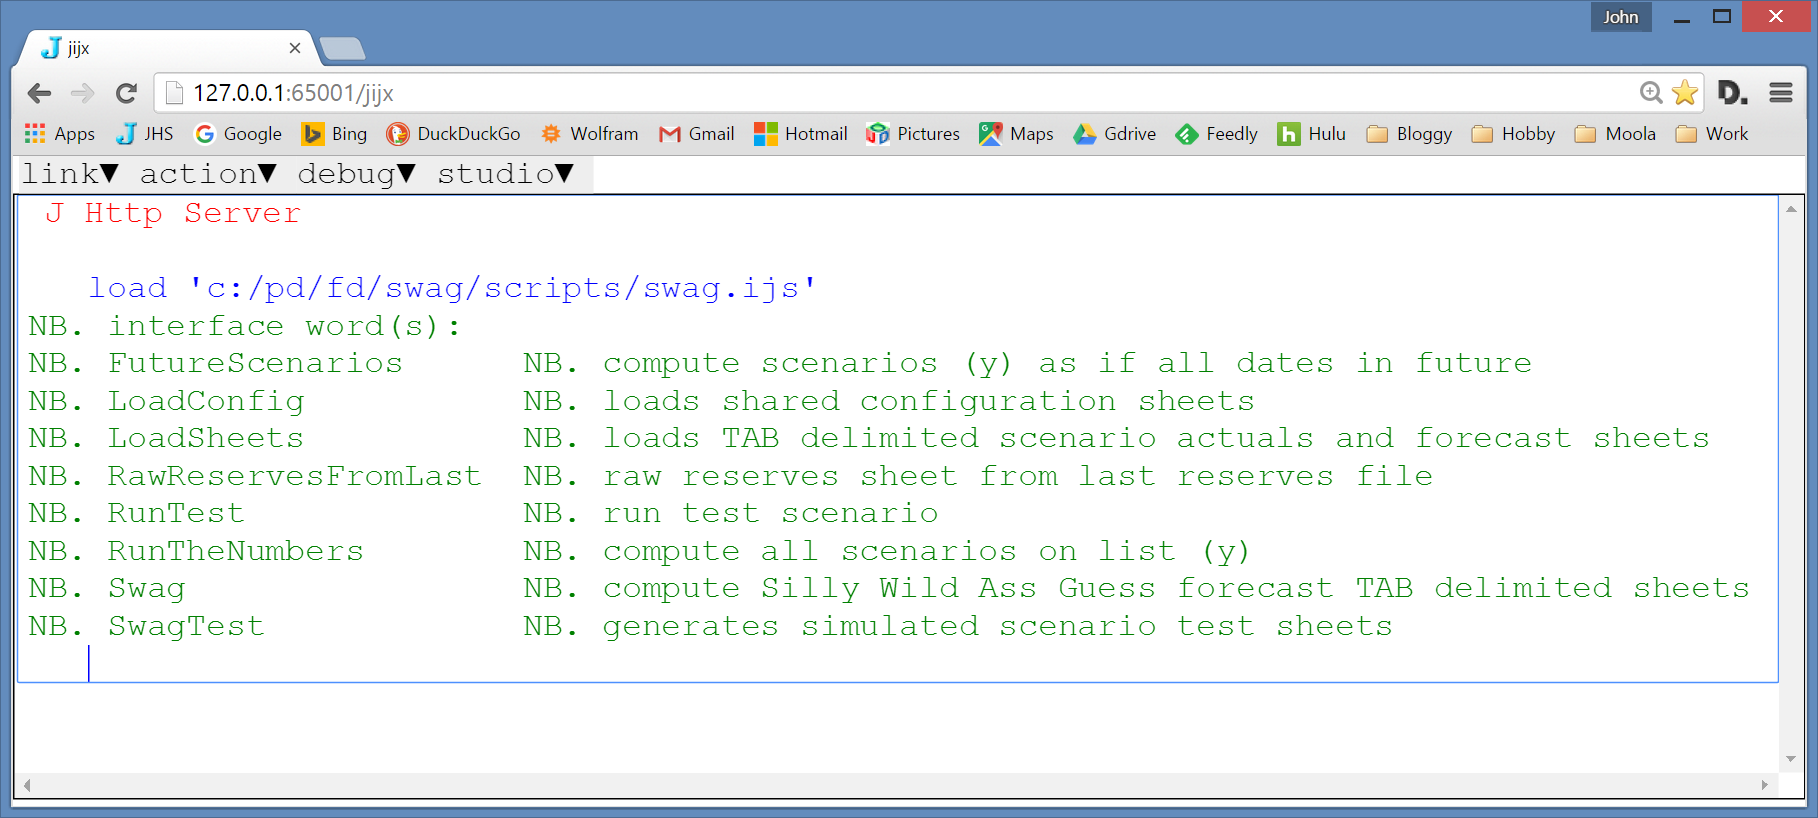
\includegraphics{jhsswag.png}\{width=``6.5in''
%height=``2.9243055555555557in''\}

\captionsetup[figure]{labelformat=empty}
\begin{figure}[htbp]
\centering
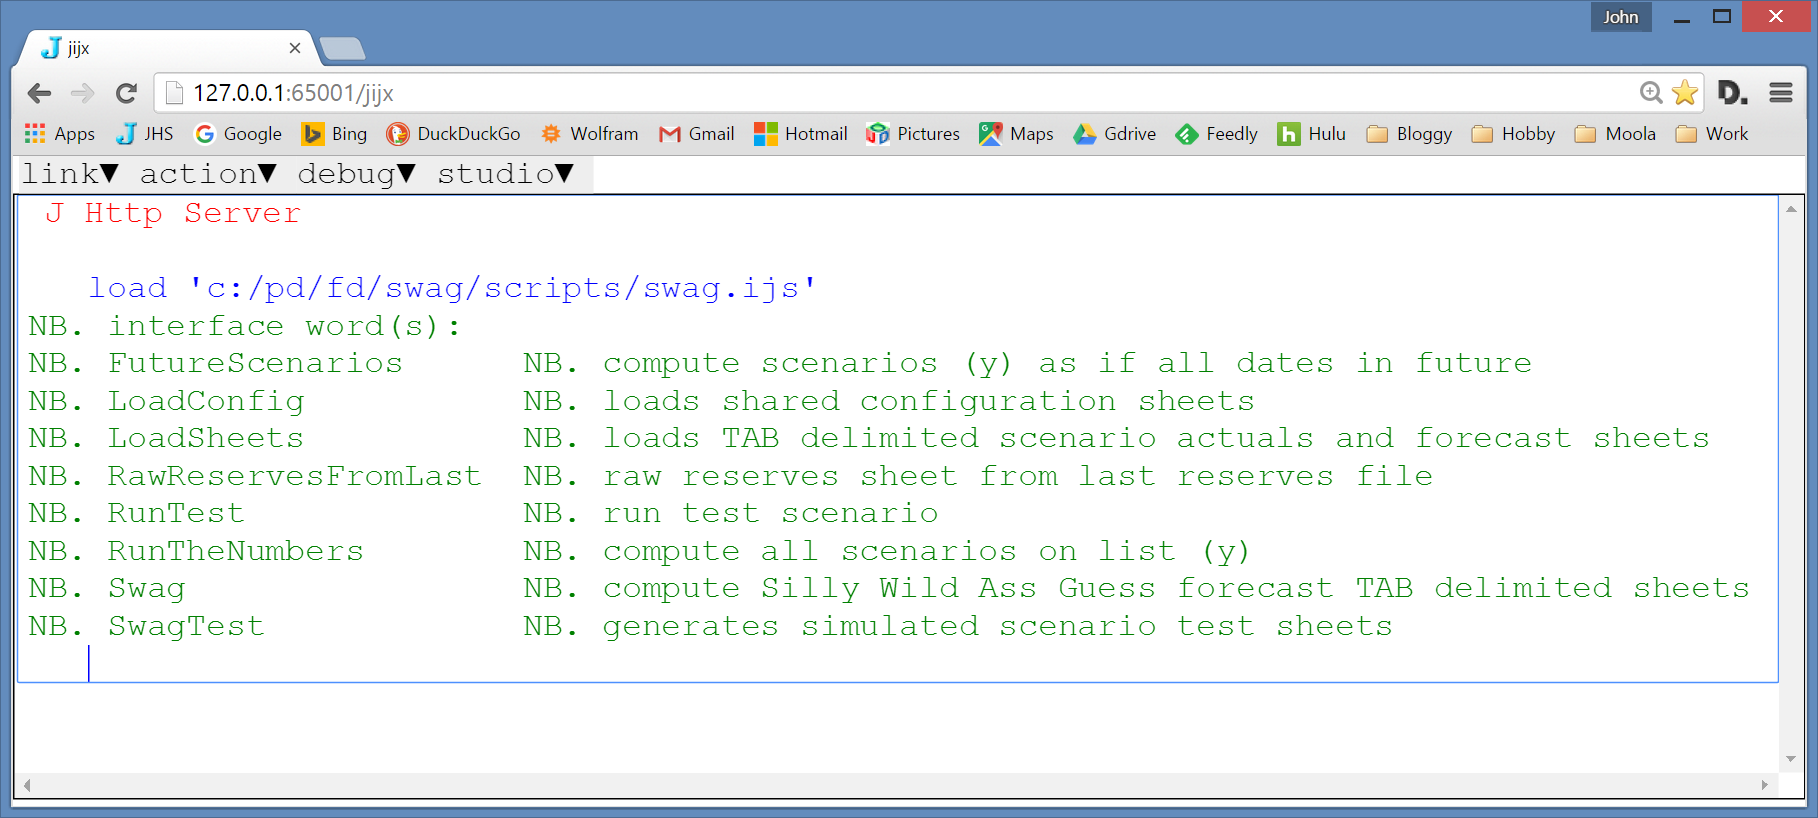
\includegraphics[width=\textwidth]{jhsswag.png}
\label{fig:5175X0}
\end{figure}

\subsection*{Execute \texttt{RunTheNumbers}}

\texttt{RunTheNumbers} sets the SWAG configuration, loads scenarios, copies
actuals to each scenario, and then evaluates each scenario. Scenarios
are numbered. I use positive numbers for ``production'' scenarios and
negative numbers for test scenarios. It sounds more complicated that it
is. This is all you have to do to execute \texttt{RunTheNumbers}

\begin{tcolorbox}[breakable, size=fbox, boxrule=1pt, pad at break*=1mm,colback=cellbackground, colframe=cellborder]
\begin{verbatim}
 RunTheNumbers 0 1 2 3 4 
\end{verbatim}
\end{tcolorbox}

\noindent The code is simple and shows what's going on.

%NOTE: lstlisting syntax coloring misses for_sn - it's a long standing problem

\begin{tcolorbox}[breakable, size=fbox, boxrule=1pt, pad at break*=1mm,colback=cellbackground, colframe=cellborder]
\begin{lstlisting}[language=jdoc, frame=single,framerule=0pt,label=lst:scr5175X0]
RunTheNumbers=:3 : 0

NB.*RunTheNumbers v-- compute all scenarios on list (y).
NB.
NB. monad:  blclFiles =. RunTheNumbers ilScenarios
NB.
NB.   RunTheNumbers 0 1 2 3 4

NB. parameters sheet is the last config sheet
ModelConfiguration_Swag_=:MainConfiguration_Swag_
parms=. ".;{:LoadConfig 0
scfx=. ScenarioPrefix

ac=. toHOST fmttd ActualSheet 0
ac write TABSheetPath,'MainActuals',SheetExt

sf=. 0$a:
for_sn. y do.
  ac write TABSheetPath,scfx,(":sn),'Actuals',SheetExt
  sf=. sf , parms Swag sn [ LoadSheets sn
end.

sf 
)
\end{lstlisting}
\end{tcolorbox}

\noindent \texttt{RunTheNumbers} writes a pair of TAB delimited forecast and
statistics files for each scenario it evaluates.

\subsection*{Open swag.xlsx and press ``Refresh All''}

The \href{https://github.com/bakerjd99/jacks/blob/master/swag/swag.xlsx}{spreadsheet \texttt{swag.xlsx}} 
loads SWAG TAB delimited text files
and plots results.\footnote{It may be necessary to adjust file paths on
  the EXCEL DATA ribbon to load SWAG TAB delimited text files.} I plot
monthly cash flow, estimated net worth and debt/equity for each
scenario. Figure~\ref{fig:5175x1} on page~\pageref{fig:5175x1} is a typical cash flow plot. It estimates mean
monthly cash balance over the scenario time range. Figure~\ref{fig:5175x2} on page~\pageref{fig:5175x2} is typical net worth plot.
It estimates mean net worth over time.

%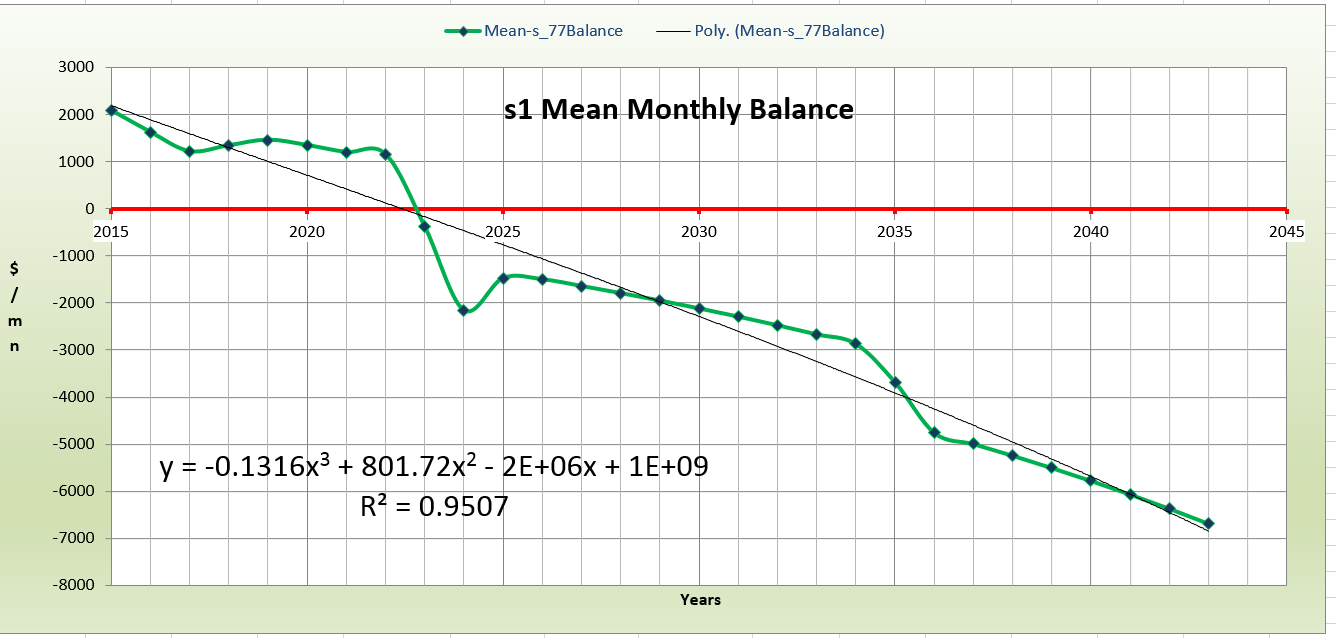
\includegraphics{meanbalance.png}\{width=``6.5in''
%height=``3.0729166666666665in''\}

\captionsetup[figure]{labelformat=default}
\begin{figure}[htbp]
\centering
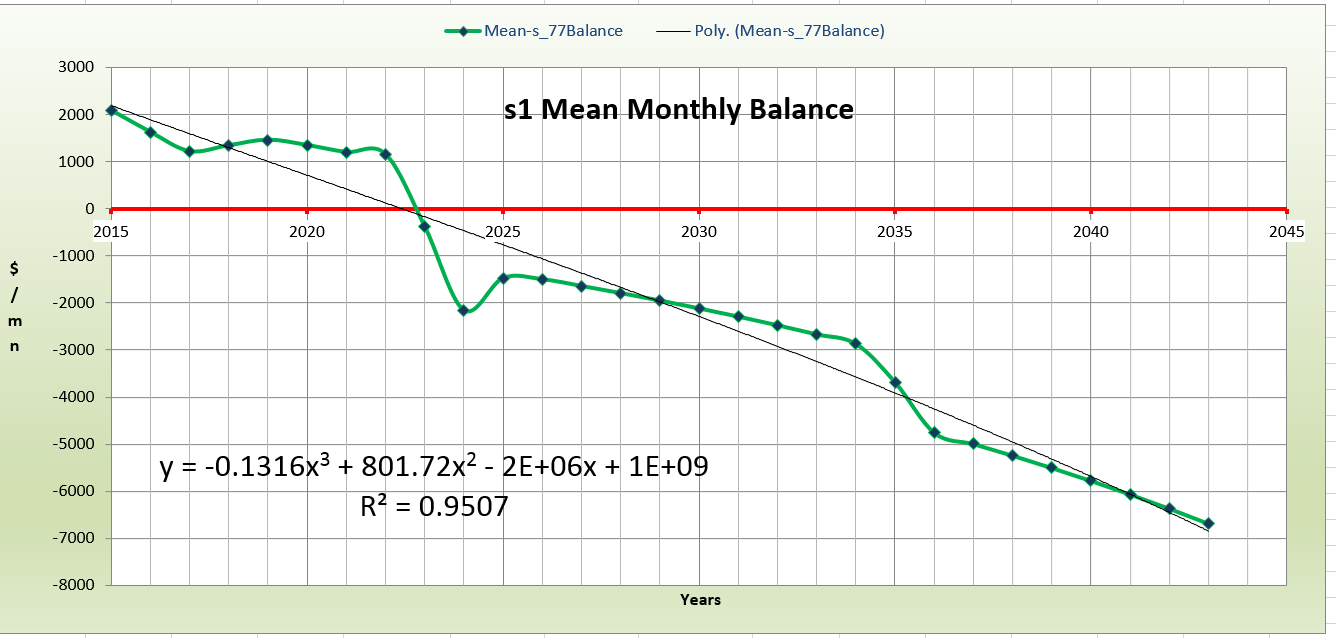
\includegraphics[width=\textwidth]{meanbalance.png}
\caption[Mean monthly cash flow balance over time. The polynomial on
the graph is an estimated trend line]{Mean monthly cash flow balance over time. The polynomial displayed on
the graph is an estimated trend line. $R^2$ is a standard fit measure.}
\label{fig:5175x1}
\end{figure}

%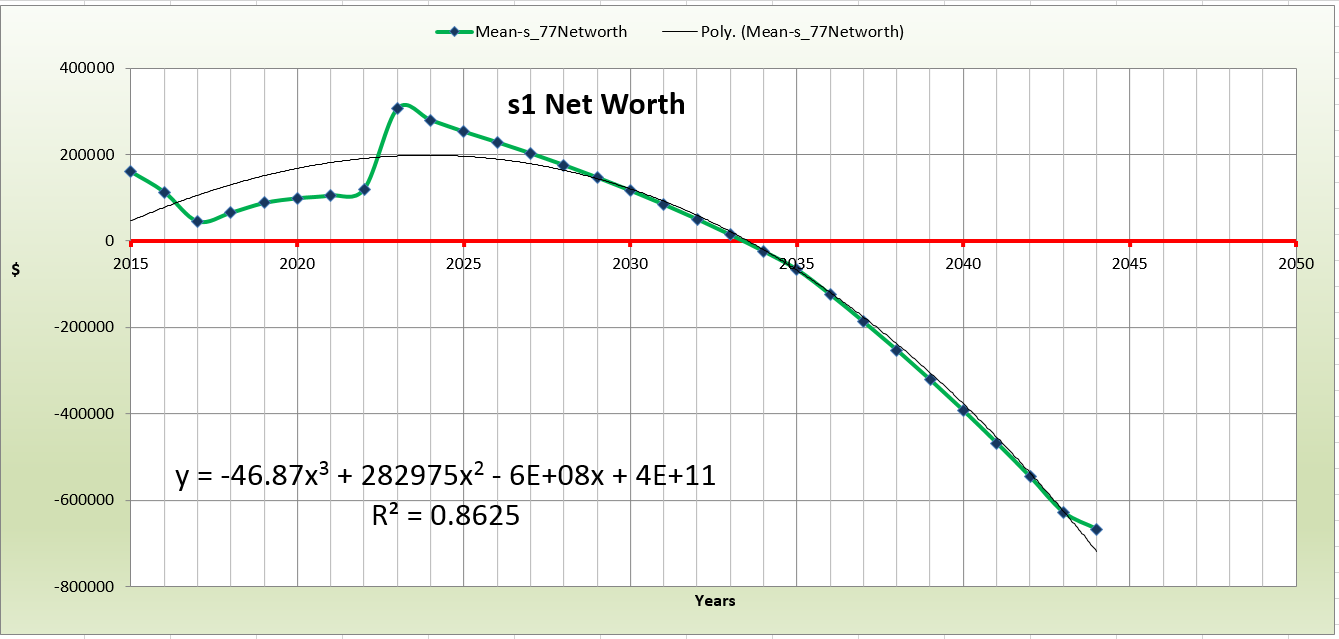
\includegraphics{networth.png}\{width=``6.5in''
%height=``3.0555555555555554in''\}

\begin{figure}[htbp]
\centering
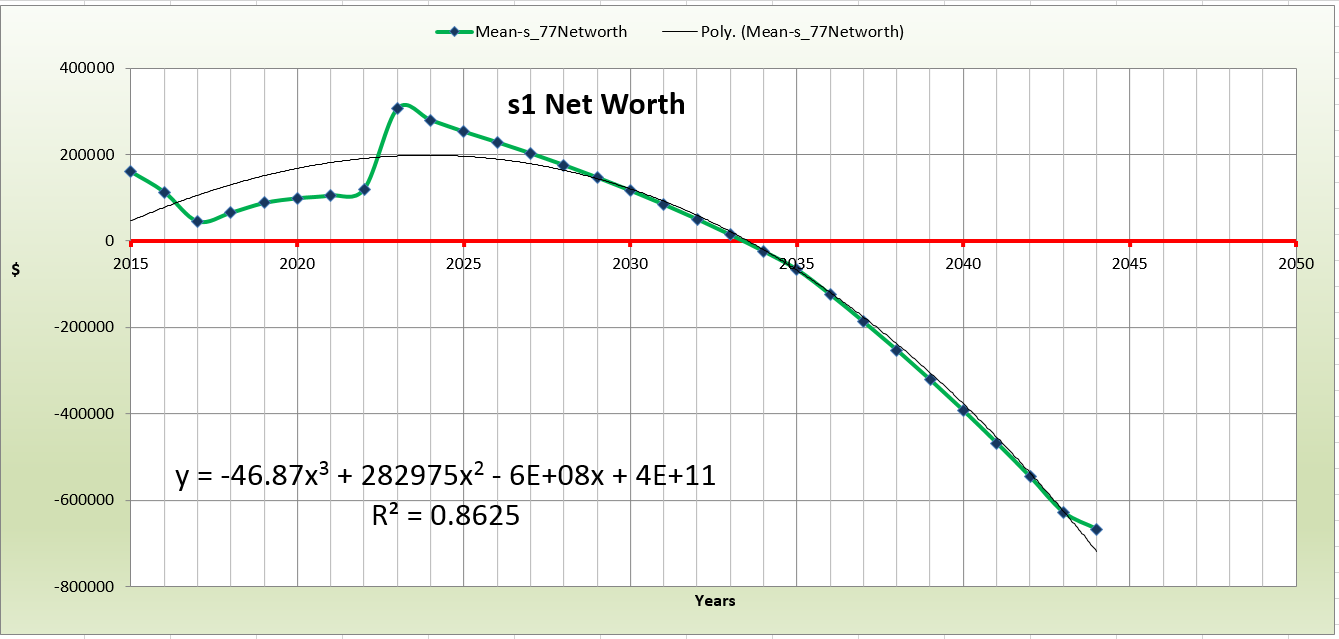
\includegraphics[width=\textwidth]{networth.png}
\caption{Mean net worth. In this happy scenario we die broke and leave a giant bill for
the government. \textit{They can meet me in Hell to collect.}}
\label{fig:5175x2}
\end{figure}


So far SWAG has met my basic needs and forced me to pay more
attention to the proverbial bottom line. As I use the system I will fix
bugs, refine rough spots, and add \emph{strictly necessary} features.
Feel free to use or adapt SWAG for your own purposes. If you do leave a
note on this blog or follow the \href{https://github.com/bakerjd99/jacks/tree/master/swag}{SWAG repository on GitHub}.

%\end{document}
